% Hi there!
% 
% This template can help you write an awesome report while focusing on its content ;-)
% I'm happy to receive your feedback at fadri.pestalozzi@gmail.com
%
% Enjoy the clear beauty and structure of LaTex!
% Fadri Pestalozzi, 2015


% In order to compile a LaTex document, we first need to load some packages
%%%%%%%%%%%%%%%%%%%%%%%%%%%%%%%%%%%%%%%%%%%%%%%%%%%%
%% first, define the document class and basic layout
%%%%%%%%%%%%%%%%%%%%%%%%%%%%%%%%%%%%%%%%%%%%%%%%%%%%
\documentclass[12pt]{report}
\usepackage[
  a4paper,    % alternative entries, feel free to experiment ^^
  twoside,    % oneside
  asymmetric, % openright
]{geometry}
% asymmetric "geometry package" to avoid swapping inner and outer marges


%%%%%%%%%%%%%%%%%%%%%%%%%%%%%%%%%%%%%%%%%%%%%%%%%%%%
%% language and characters
%%%%%%%%%%%%%%%%%%%%%%%%%%%%%%%%%%%%%%%%%%%%%%%%%%%%

% switch language-specific output to German
% for example: "Contents" becomes "Inhaltsverzeichnis"
%\usepackage[ngerman]{babel}

% load a font containing most common characters
\usepackage{lmodern}

% Zur Verwendung von Umlauten im Text wird das Paket "inputenc" benötigt
\usepackage[utf8]{inputenc}

% Zum Trennen von Wörtern mit Umlauten wird das Paket "fontenc" benötigt
\usepackage[T1]{fontenc}

\usepackage{amsmath}	% need for subequations and characters like \backslash to depict "\"

%%%%%%%%%%%%%%%%%%%%%%%%%%%%%%%%%%%%%%%%%%%%%%%%%
%% extend numbering in table of contents
%%%%%%%%%%%%%%%%%%%%%%%%%%%%%%%%%%%%%%%%%%%%%%%%%

% subsubsection number visible, paragraph without number
%\setcounter{secnumdepth}{3}   
%\setcounter{tocdepth}{3}		% include into toc

% paragraph number visible
%\setcounter{secnumdepth}{4}  
%\setcounter{tocdepth}{4}    	% include into toc


%%%%%%%%%%%%%%%%%%%%%%%%%%%%%%%%%%%%%%%%%%%%%%%%%%%%
%% customize page headers and footers
%%%%%%%%%%%%%%%%%%%%%%%%%%%%%%%%%%%%%%%%%%%%%%%%%%%%
\usepackage{fancyhdr} % place text on the top and/or bottom of every page

\pagestyle{fancy}     % style further defined in layout.tex
\fancyhf{}            % Kopf- und Fusszeile leeren
\fancyhead[RO,LE]{\leftmark}  % R=right, L=left, O=odd, E=even, \leftmark = chapter, \rightmark = section
%\fancyhead[LO,RE]{\rightmark}
\fancyfoot[C]{\thepage}
\renewcommand\headrulewidth{0.4pt}
\renewcommand\footrulewidth{0.0pt}

\setlength{\headheight}{15pt} % fancyhdr requires headheight to be at least 15pt


% Put this at the end of the preamble to avoid that LaTex forces chapters to always start on even pages
\renewcommand{\cleardoublepage}{\clearpage}

% to convert "chapter # // name" into "# name" --> use \titleformat & to do so, first load the package titlesec
\usepackage{titlesec} % Textüberschriften anpassen
\titleformat{\chapter}[hang]{\normalfont\Large\bf}{\LARGE\bf\thechapter}{1ex}{\LARGE}

%%%%%%%%%%%%%%%%%%%%%%%%%%%%%%%%%%%%%%%%%%%%%%%%%%%%
%% customization of line spacing and page layout
%%%%%%%%%%%%%%%%%%%%%%%%%%%%%%%%%%%%%%%%%%%%%%%%%%%%
%\setlength{\baselineskip}{16.0pt}    % 16 pt usual spacing between lines
%\setlength{\parskip}{3pt plus 2pt}
%\setlength{\parindent}{20pt}
%\setlength{\oddsidemargin}{0.5cm}
%\setlength{\evensidemargin}{0.5cm}
%\setlength{\marginparsep}{0.75cm}
%\setlength{\marginparwidth}{2.5cm}
%\setlength{\marginparpush}{1.0cm}
%\setlength{\textwidth}{150mm}


%%%%%%%%%%%%%%%%%%%%%%
%% distance of chapter heading reduced
%%%%%%%%%%%%%%%%%%%%%%
\titlespacing{\chapter}{0pt}{1em}{12pt}

%%% intuitive Syntax
%\titleformat{Überschriftenklasse}[Absatzformatierung]{Textformatierung} {Nummerierung}{Abstand zwischen Nummerierung und Überschriftentext}{Code vor der Überschrift}[Code nach der Überschrift]
%\titleformat{\chapter}[hang]{\large\bfseries}{\thechapter\quad}{0pt}{}
%\titleformat{\section}[hang]{\large\bfseries}{\thesection\quad}{0pt}{}
%\titleformat{\subsection}[hang]{\large\bfseries}{\thesubsection\quad}{0pt}{}
%\titleformat{\subsubsection}[hang]{\large\bfseries}{\thesubsubsection\quad}{0pt}{}
%\titleformat{\paragraph}[hang]{\large\bfseries}{\theparagraph\quad}{0pt}{}

%%% exakte Syntax
%\titlespacing{Überschriftenklasse}{Linker Einzug}{Platz oberhalb}{Platz unterhalb}[rechter Einzug]
%\titlespacing{\section}{0pt}{6pt}{6pt}
%\titlespacing{\subsection}{0pt}{6pt}{6pt}
%\titlespacing{\subsubsection}{0pt}{6pt}{6pt}
%\titlespacing{\paragraph}{0pt}{6pt}{6pt}


%%%%%%%%%%%%%%%%%%%%%%%%%%%%%%%%%%%%%%%%%%%%%%%%%%%%
%% text
%%%%%%%%%%%%%%%%%%%%%%%%%%%%%%%%%%%%%%%%%%%%%%%%%%%%
\usepackage{lipsum}  % to generate dummy text
% Syntax inside document:
% \lipsum            % default = slightly more than a single page
% \lipsum[3-56]      % generate an arbitrary number of paragraphs

\usepackage{color}    % use colored text, e.g. to highlight "work in progress"
% Syntax inside document:
% \textcolor{red}{colored_text}

% subscript and supterscripts ??
% \textsubscript{}
% \textsuperscript{}

% Non-breaking space to prevent the processor from inserting a line break
% D.~\textsc{Knuth}

%%%%%%%%%%%%%%%%%%%%%%%%%%%%%%%%%%%%%%%%%%%%%%%%%%%%
%% tables
%%%%%%%%%%%%%%%%%%%%%%%%%%%%%%%%%%%%%%%%%%%%%%%%%%%%

% enable drawing horizontal lines (hline) across specific columns
% \toprule
% \midrule
% \bottomrule
% example to draw midrule between selected columns 2 and 3
% .. & .. & .. \\ \cmidrule{2-3}
\usepackage{booktabs}  

%% enable long tables, exceeding one page
%\usepackage{longtable}
%
%% use cells merged between adjacent columns
%% mehrzeilige Tabelleneinträge
%\usepackage{multirow}

%%%%%%%%%%%%%%%%%%%%%%%%%%%%%%%%%%%%%%%%%%%%%%%%%%%%
%% figures
%%%%%%%%%%%%%%%%%%%%%%%%%%%%%%%%%%%%%%%%%%%%%%%%%%%%
\usepackage{graphicx}   % need for figures

\usepackage{caption}	% to add captions to figures or tables

\usepackage{subcaption} % use subcaption package to put several images inside the same figure (subfigure-package is outdated. BUT the command is still called "subfigure" ^^

\usepackage{here}       % to enforce the figure start with a capital "H" -> "\begin{figure}[H]"  Without this, LaTex looks for a suitable spot to place a figure.

%%%%%%%%%%%%%%%%%%%%%%%%%%%%%%%%%%%%%%%%%%%%%%%%%%%%
%% logo
%%%%%%%%%%%%%%%%%%%%%%%%%%%%%%%%%%%%%%%%%%%%%%%%%%%%
\usepackage{eso-pic}    % to place figures outside text margins (e.g. to include a logo). 

%%%%%%%%%%%%%%%%%%%%%%%%%%%%
% define positions for logos
%%%%%%%%%%%%%%%%%%%%%%%%%%%%

% upper left
\newcommand\AtPageMyUpperLeft[1]{\AtPageLowerLeft{%
% \put(x,y) zero position at lower left corner of page
\put(\LenToUnit{0.1\paperwidth},\LenToUnit{0.85\paperheight}){#1}}}

% upper right
\newcommand\AtPageMyUpperRight[1]{\AtPageLowerLeft{%
% \put(x,y) zero position at lower left corner of page
\put(\LenToUnit{0.75\paperwidth},\LenToUnit{0.85\paperheight}){#1}}}

%%%%%%%%%%%%%%%%%%%%%%%%%%%%
% define logos
%%%%%%%%%%%%%%%%%%%%%%%%%%%%

% upper left
\AddToShipoutPicture*{ % * ensures placement on first page only
  \AtPageMyUpperLeft{
  	{
\includegraphics[height=3cm,keepaspectratio]{files/images/logo-LaTeX.jpg}}}}

% upper right
\AddToShipoutPicture*{ % * ensures placement on first page only
  \AtPageMyUpperRight{
  	{
\includegraphics[height=3cm,keepaspectratio]{files/images/logo-GitHub.jpg}}}}

%%%%%%%%%%%%%%%%%%%%%%%%%%%%
% further logo handling
%%%%%%%%%%%%%%%%%%%%%%%%%%%%

% to place image on every page instead of only first one, remove star
% i.e. \AddToShipoutPicture{..} 

% using \AddToShipoutPicture{..}, the printing can be stopped on further pages by calling \ClearShipoutPicture



%%%%%%%%%%%%%%%%%%%%%%%%%%%%%%%%%%%%%%%%%%%%%%%%%%%%
%% hyperlinks
%%%%%%%%%%%%%%%%%%%%%%%%%%%%%%%%%%%%%%%%%%%%%%%%%%%%

% to break long urls at hyphens and spaces, call before {hyperref}-package
\usepackage[hyphens,obeyspaces,spaces]{url}  

% hypertext links, including those to external documents and URLs
\usepackage[hidelinks,bookmarks,colorlinks=false]{hyperref} % for pdf hyperlinks, hidelinks==suppress printing a border around the links

% adjust figure-links to point to the figure instead of the caption below
\usepackage[all]{hypcap}            
% vertical distance adjustment for links to figure captions
\renewcommand{\hypcapspace}{100pt}  


%%%%%%%%%%%%%%%%%%%%%%%%%%%%%%%%%%%%%%%%%%%%%%%%%%%%
%% nomenclature / list of acronyms
%%%%%%%%%%%%%%%%%%%%%%%%%%%%%%%%%%%%%%%%%%%%%%%%%%%%
\usepackage{nomencl}                % in order to include a nomenclature
\usepackage[printonlyused,withpage]{acronym} % "printonlyused" to hide entries which are not used. "withpage" includes the page where the acronym is used


%% define a german label for the nomenclature
%\renewcommand{\nomname}{Abkürzungsverzeichnis}
%
%%% Abkürzung und Erklärung mittels horizontaler Punktlinie verbinden
%\setlength{\nomlabelwidth}{.20\hsize}
%\renewcommand{\nomlabel}[1]{#1 \dotfill}
%
%%%% Zeilenabstände verkleinern
%\setlength{\nomitemsep}{-\parsep}
%\makenomenclature


%%%%%%%%%%%%%%%%%%%%%%%%%%%%%%%%%%%%%%%%%%%%%%%%%%%%
%% show tex-code in LaTeX pdf-document
%%%%%%%%%%%%%%%%%%%%%%%%%%%%%%%%%%%%%%%%%%%%%%%%%%%%

\usepackage{listings}
% \usepackage[usenames,dvipsnames]{color}  % for optional color RoyalBlue

% syntax to display latex code in pdf output:
% \begin{document}
% \lstinputlisting{files/code-2-display.tex}
% \end{document}

% optional settings to customize layout of listing output
% call \lstset{..} inside header, i.e. just next to \usepackage{listings}
% 
% listings settings from classicthesis package by
% Andr\'{e} Miede
%\lstset{language=[LaTeX]Tex,%C++,
%    keywordstyle=\color{RoyalBlue},%\bfseries,
%    basicstyle=\small\ttfamily,
%    %identifierstyle=\color{NavyBlue},
%    commentstyle=\color{Green}\ttfamily,
%    stringstyle=\rmfamily,
%    numbers=none,%left,%
%    numberstyle=\scriptsize,%\tiny
%    stepnumber=5,
%    numbersep=8pt,
%    showstringspaces=false,
%    breaklines=true,
%    frameround=ftff,
%    frame=single
%    %frame=L
%}

\lstset{language=[LaTeX]Tex,%C++,
    %keywordstyle=\color{RoyalBlue},%\bfseries,
    %basicstyle=\small\ttfamily,
    %identifierstyle=\color{NavyBlue},
    %commentstyle=\color{Green}, %\ttfamily,
    %stringstyle=\rmfamily,
    %numbers=none,%left,%
    %numberstyle=\scriptsize,%\tiny
    %stepnumber=5,
    %numbersep=8pt,
    %showstringspaces=false,
    breaklines=true %,
    %frameround=ftff,
    %frame=single
    %frame=L
}

%%%%%%%%%%%%%%%%%%%%%%%%%%%%%%%%%%%%%%%%%%%%%%%%%%%%
%% bibliography
%% To avoid compilation errors load bibliography package as last package
%%%%%%%%%%%%%%%%%%%%%%%%%%%%%%%%%%%%%%%%%%%%%%%%%%%%
\usepackage[nottoc,notlof,notlot]{tocbibind} 	% tocbibind = Put the bibliography in the table of contents





% Frequently used content (e.g. symbols, formulas, environments, ...) can be replaced by customized commands for more efficient writing

%===================================================================
%======================= CUSTOMIZED COMMANDS =======================
%===================================================================

% If a punctuation character like "." or "," follows a customized command, we need to omit the blank space otherwise necessary.
% To solve this dilemma we can introduce the d-form of any command, where no space is printed afterwards. "d" stands for "dot".

% As some very short commands like \g are reserved by LaTex, we can describe any unit by simply starting off with a "u".


%%%%%%%%%%%%%%%%%%%%%%%%%%%% Arrows %%%%%%%%%%%%%%%%%%%%%%%%%%%%%%%

\newcommand{\ua}{$\uparrow$ }
\newcommand{\da}{$\downarrow$ }
\newcommand{\ra}{$\rightarrow$ }
\newcommand{\la}{$\leftarrow$ }

%%%%%%%%%%%%%%%%%%%%%%%%%%% Percent %%%%%%%%%%%%%%%%%%%%%%%%%%%%%%%

\newcommand{\upc}{$\%$ }
\newcommand{\upcd}{$\%$}

%%%%%%%%%%%%%%%%%%%%%%%%% Temperature %%%%%%%%%%%%%%%%%%%%%%%%%%%%%

\newcommand{\ucels}{$^\circ \mathrm{{C}}$ }
\newcommand{\ucelsd}{$^\circ \mathrm{{C}}$}


%%%%%%%%%%%%%%%%%%%%%%%%%%%%% Weight %%%%%%%%%%%%%%%%%%%%%%%%%%%%%%%

\newcommand{\ug}{$\mathrm{g}$ }
\newcommand{\ugd}{$\mathrm{g}$}

\newcommand{\umg}{$\mathrm{mg}$ }
\newcommand{\umgd}{$\mathrm{mg}$}


%%%%%%%%%%%%%%%%%%%%%%%%%%%%%% Time %%%%%%%%%%%%%%%%%%%%%%%%%%%%%%%%

\newcommand{\us}{$\mathrm{s}$ }
\newcommand{\usd}{$\mathrm{s}$}

\newcommand{\umin}{$\mathrm{min}$ }
\newcommand{\umind}{$\mathrm{min}$}

\newcommand{\uh}{$\mathrm{h}$ }
\newcommand{\uhd}{$\mathrm{h}$}

%%%%%%%%%%%%%%%%%%%%%%%%%%%%% Length %%%%%%%%%%%%%%%%%%%%%%%%%%%%%%%

\newcommand{\um}{$\mathrm{m}$ }
\newcommand{\umd}{$\mathrm{m}$}

\newcommand{\umm}{$\mathrm{mm}$ }
\newcommand{\ummd}{$\mathrm{mm}$}

\newcommand{\umu}{$\mathrm{\mu m}$ }
\newcommand{\umud}{$\mathrm{\mu m}$}

%%%%%%%%%%%%%%%%%%%%%%%%%%% Chemistry %%%%%%%%%%%%%%%%%%%%%%%%%%%%%%

\newcommand{\coo}{$\mathrm{CO_2}$ }
\newcommand{\cood}{$\mathrm{CO_2}$}

\newcommand{\hh}{$\mathrm{H_2}$ }
\newcommand{\hhd}{$\mathrm{H_2}$}


%%%%%%%%%%%%%%%%%%%%%%% Math Environment %%%%%%%%%%%%%%%%%%%%%%%%%%

\newcommand{\di}{\displaystyle}   % to present important formulas with a nice big font


%%%%%%%%%%%%%%%%%%%%%%%%%%%% Colors %%%%%%%%%%%%%%%%%%%%%%%%%%%%%%%%

\newcommand{\todo}{\textcolor{red}{Pendent! }}

% define color to track work progress, can be set to black=000 at the end of the work
\definecolor{progress_color}{rgb}{1,0,0}

% use color for new command \re = red = review = work in progress
\newcommand{\re}{\textcolor{progress_color}}

% usage in text:
% \re{statement in red}

% After loading packages and defining commands, we can now start writing the actual document
\begin{document}

% To separate introductory content from bulk text, I like to start off using roman page numbering. The default page numbering uses arabic numbers.
\pagenumbering{roman}

% Let's start by creating a custom title page
\thispagestyle{empty} 	% begin from scratch

\begin{center}

% logos created inside packages.tex

\vspace*{7cm}

\huge{\textbf{Another awesome LaTex Report}}

\vspace{1.5cm}

\Large Brought to you by:

\vspace{0.7cm}

\huge{\textbf{Slurm!}}

\vspace{0.7cm}

\Large The world's ooziest soft drink.

\vfill

\Large Slurms McKenzie
\\ % \\ = new line
\Large January 3007


\end{center}



% To continue on a fresh page after finishing the table of contents, break the page!
\pagebreak

\hypertarget{toc:label}{}  %second brackets could hold target text. 
%empty target label to refer to the table of contents

% Next off, we can create a table of contents. The LaTex "table of contents" is automatically hyperlinked to the content listed inside. After following a link inside the pdf, jump back using alt+ArrowKeyLeft
\tableofcontents

\pagebreak

% Switching back to arabic page numbering for the main text
\pagenumbering{arabic}

% Input individual chapters or even sections as separate .tex files for more clarity
\chapter{Chapter Title}

This chapter contains examples of LaTeX code in action.
To look at and work with the underlying templates, switch to the corresponding position in the .tex file by hitting "Ctrl + LeftClick" here, i.e. inside the Pdf Viewer of Texmaker.

\section{Section Title}

Chapters are divided into sections.

\subsection{Subsection Title}
\label{text:subsection}
Sections are further divided into subsections.

\subsubsection{Subsubsection Title}
For even finer subdivision of text you can add another sub-prefix.

\paragraph{Paragraph Title}

A paragraph is the lowest level of text subdivision. 
Note that the paragraph title is put in line with the bulk text.

\section{Automatic Numbering}

For any new definition, LaTeX creates an automatic numbering.
This applies to text structures like chapters, sections and paragraphs, as well as to additional environments like tables, figures and equations.
Examples can be found in table \ref{tab:keyboard-shorts}, figure \ref{fig:xkcd} and equation ??.

By default, the text numbering is active down to subsection level, as shown in subsection \ref{text:subsection} above.

By the way: Did you notice how the mouse pointer changes to a hand symbol when hovering over the subsection number above?
Whenever the hand symbol is visible, you are pointing onto a dynamic link, which can be used to jump to the corresponding label.

\subsection{Extend Numbering to Lower Levels}

If additional sub-levels need to be numbered, include one of the two following code snippets into the header file "packages.tex".

To number down to subsubsections but leave paragraphs without number:
\lstinputlisting{files/chapters/chapter-1-sections/extend-numbering-lvl3-subsubsections.tex}

To number paragraphs as well:
\lstinputlisting{files/chapters/chapter-1-sections/extend-numbering-lvl4-paragraphs.tex}


\section{Label for a Reference}

To refer to a specific position inside a LaTeX report, declare a label.
\label{text:a-label-position}
This label is only visible in the LaTeX editor and not printed into the final pdf. To find the hidden label in this section, hit "Alt+LeftClick" right here inside the "Pdf Viewer".

Labels can be placed in special environments like tables, figures and equations as well.

\section{Reference to a Label}

As seen in section \ref{text:a-label-position}, a reference needs a label to work.
Inside the pdf generated by LaTeX, you can click on any reference to jump to the corresponding label position.
This possibility is visualized by the mouse pointer changing to a hand symbol with one finger pointing upward.

\hyperlink{toc:label}{It's also possible to customize links, e.g. to jump to the table of contents.}

\subsection{Jump Back to Label Position}

After following a link inside the output pdf, you can press "Alt+LeftArrow" to jump back to the original position inside the pdf.
For this feature to work, the pdf has to be opened outside the Texmaker program, e.g. with the \url{https://get.adobe.com/reader/}.


\section{Commenting}

To write a comment in your .tex file, start a new line with "\%".
Commented code parts are ignored by the compiler.


\section{Include .tex Files}
\label{text:include-files}




\section{Figure}

\subsection{Single Image}

% {figure}[H] or {figure}[htb]
% [H] enforces the figure to be exactly here
% [htb] allows the figure to be placed either here, on top or at the bottom of the page. Checking for suitable location in this order (first h, 2nd t, last b).

\begin{figure}[H]
  \begin{center}
    % \includegraphics[attr1=val1, attr2=val2, ...]{imagepath/imagename}
    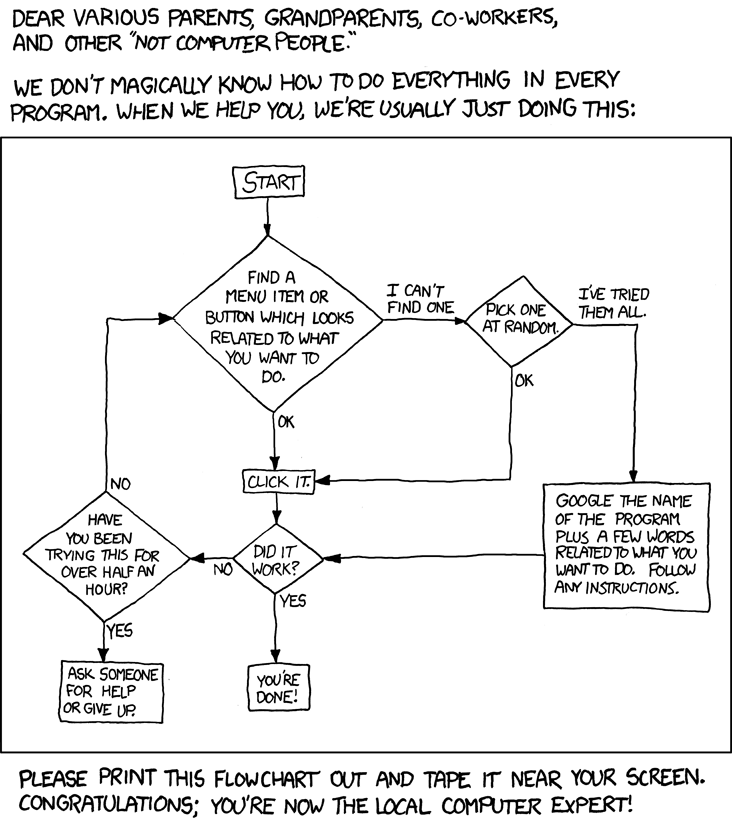
\includegraphics[width=0.75\columnwidth]{files/images/xkcd_tech_support_cheat_sheet.png}
  \end{center}
  \caption{On how to become a local computer expert. \\ Don't forget "Ctrl+LeftClick" here :) }
  % \\ = new line
  % call caption before label
  \label{fig:xkcd}
\end{figure}


\subsection{Multiple Images}




\section{Citation}

To cite bibliography sources in LaTeX, I recommend using JabRef. 
JabRef is an open source graphical application for managing bibliographical data.

Besides standard citations like books \cite{2000_Kuffel_HV_engineering_fundamentals} or articles \cite{2004_Whitesides_writing_a_paper}, JabRef can also be used to define custom entry types like webpages for example \cite{2015_github_webpage}.


\section{Nomenclature Entries}

Technical terms and abbreviations used inside a report can be gathered using a nomenclature (see section \ref{text:nomenclature}).

Define new nomenclature entry, e.g. a specific abbreviation, inside the separate file nomenclature.tex 

ref ??.
This definition can then be linked to usages of the technical term inside the report.
%\phantomsection \label{def:tg}
%Thermogravimetric measurements are performed with a \acs{tg}.

%\subsection{subsection name}
%
%To address the diffusion limitations encountered by \acs{tg}, a packed bed tubular reactor (\phantomsection \label{def:pb} \acs{pb}) has been developed. \lipsum[2] 


\section{Switch to German Output Language}

Switch language-specific output to German by calling:

\lstinputlisting{files/chapters/chapter-1-sections/switch-language-to-german.tex}

 as the first package in the header file "packages.tex".
As an example, "Contents" then becomes "Inhaltsverzeichnis" and "Bibliography" becomes "Quellenverzeichnis".


\section{Filler Text}

Here's an example of filler text, e.g. to test the appearance of a new font setting.

\lipsum[1]

\section*{Suppress Numbering}
\addcontentsline{toc}{section}{Suppress Numbering}

To suppress numbering of a particular LaTeX object add "*" between object call and curly brackets.
As an example, the current section was created by:

\lstinputlisting{files/chapters/chapter-1-sections/suppress-numbering.tex}

This can be useful to separate certain parts like the nomenclature or appendix from the main text.
Suppressing the numbering also prevents enumeration in the table of contents. 
To still create an entry in the \hyperlink{toc:label}{table of contents}, call the following code just after creating the suppressed section:

\lstinputlisting{files/chapters/chapter-1-sections/suppress-numbering-into-toc.tex}

\chapter{Another Chapter Title}

For a better overview and structured writing, I recommend you place each chapter into a separate .tex file.
As shown in section \ref{text:include-files}, further subdivision of the .tex code is possible if necessary.

\section{Table, Texmaker Keyboard Shortcuts}

For more efficient work with Texmaker, the keyboard shortcuts in table \ref{tab:keyboard-shorts} come in handy.

% Table generated by Excel2LaTeX from sheet 'keyboard-shortcuts'
\begin{table}[htbp]
  \centering

  % \caption{Add caption}
  %% automatic caption created by Excel2Latex is positioned on top of the table
  %% to instead position a caption after the table see below (*)

    \begin{tabular}{ll}
    \toprule
    keyboard shortcut & action triggered \\
    \midrule
    \multicolumn{1}{r}{} & \multicolumn{1}{r}{} \\
    \multicolumn{2}{l}{\textbf{startup procedure}} \\
    Ctrl + Shift + F8 & open files and master from last session \\
    F1    & compile \\
          &  \\
    \multicolumn{2}{l}{\textbf{file navigation}} \\
    Ctrl + F, M & find, find next \\
    Alt + Page Up/Down & switch between open .tex-files \\
    Ctrl + LeftClick in Pdf Viewer & jump to corresponding point in editor \\
          &  \\
    \multicolumn{2}{l}{\textbf{commenting}} \\
    Ctrl + T & comment selected code \\
    Ctrl + U & uncomment selected code \\
    \bottomrule
    \end{tabular}%

	% (*) new caption position below tabular environment, label afterwards!
	\caption{Add caption}
    % within a table, the label has to be called after the caption
    % otherwise there will be a compilation error
	\label{tab:keyboard-shorts}

\end{table}%


The above table is included as a separate .tex file, as described in \ref{text:include-files}.


\section{Packages}

%\usepackage[option1,option2]{package_name}

\section{Error Messages}

This section contains common error messages when compiling .tex into .pdf.
To display possible error messages, activate the window "Messages/Log" within the Texmaker editor as shown in figure \ref{fig:texmaker-messages-log}.

When encountering a new error message, it makes sense to compile once more.
Some errors are caused by incompatibilities between intermediate compilation files and newly written .tex-code. In such a case, recompilation can eliminate those error messages.

\subsection{overfull vbox}

%\lstinputlisting{files/chapters/chapter-2-sections/error-message-overfull-vbox.tex}

%\backslash
"overfull  vbox" means you have too much stuff on a page for LaTeX to arrange nicely. Consider either reducing the size of figures or removing the [H] enforcing the figure to be placed "Here".

%"underfull \vbox" means you have not enough stuff on a page for LaTex to arrange nicely
% consider adding a \pagebreak or \newpage to fill up of extra vertical space

% if "underfull" is the result from a url being too long, add "\hfill" to the corresponding bibtex entry


% TESTING
% Copy the following skeleton report into a standalone .tex file and compile for quick testing

%\documentclass[preview,border=12pt,varwidth]{standalone}
%% \usepackage{optional_package_to_include_inside_the_test}
%
%\begin{document}
%
%test
%
%\end{document}


%
%
%
%\phantomsection \label{def:eps}
%As the permittivity \acs{eps} increases, so does the ability of a given material to attract high voltage breakdown events. \lipsum[3]
%
%
%\section{include sub files}
%
%\input{files/chapters/chapter_2_sections/Molare_Masse}
%
%\section{section name}
%
%\subsection{subsection name}
%
%As shown in chapter \ref{ch:fourty_two}, a subcaption example is still missing:
%
%\begin{figure}
%        \centering
%        \begin{subfigure}[b]{0.3\textwidth}
%                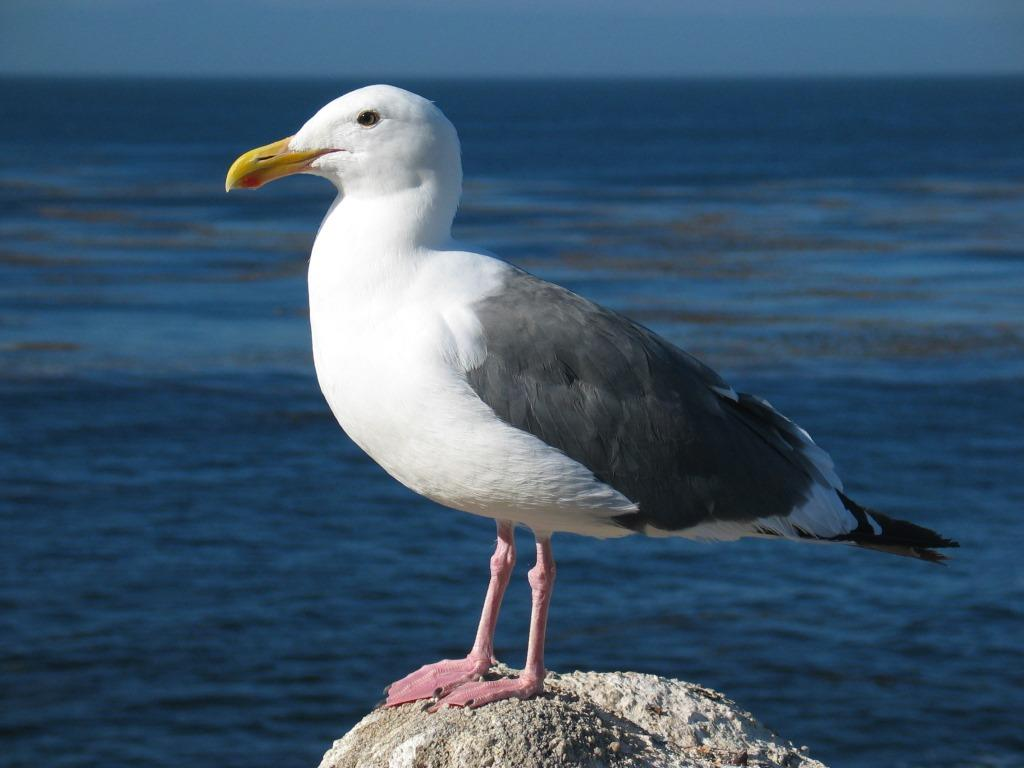
\includegraphics[width=\textwidth]{files/images/gull}
%                \caption{A gull}
%                \label{fig:gull}
%        \end{subfigure}%
%        ~ %add desired spacing between images, e. g. ~, \quad, \qquad, \hfill etc.
%          %(or a blank line to force the subfigure onto a new line)
%        \begin{subfigure}[b]{0.3\textwidth}
%                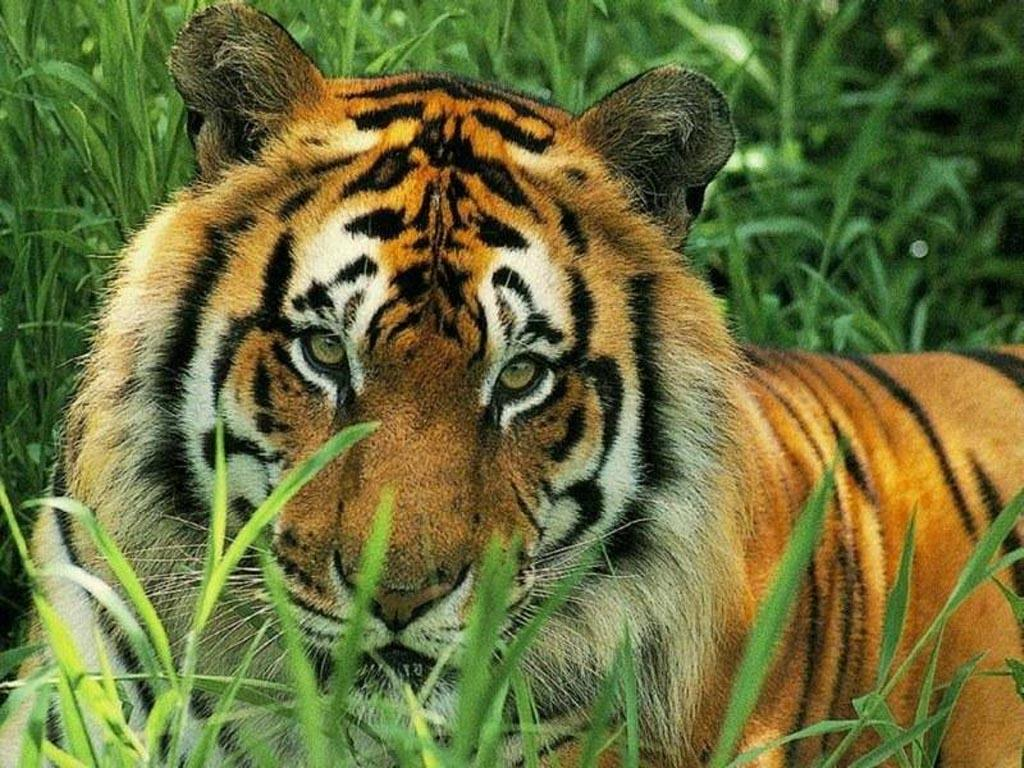
\includegraphics[width=\textwidth]{files/images/tiger}
%                \caption{A tiger}
%                \label{fig:tiger}
%        \end{subfigure}
%        ~ %add desired spacing between images, e. g. ~, \quad, \qquad, \hfill etc.
%          %(or a blank line to force the subfigure onto a new line)
%        \begin{subfigure}[b]{0.3\textwidth}
%                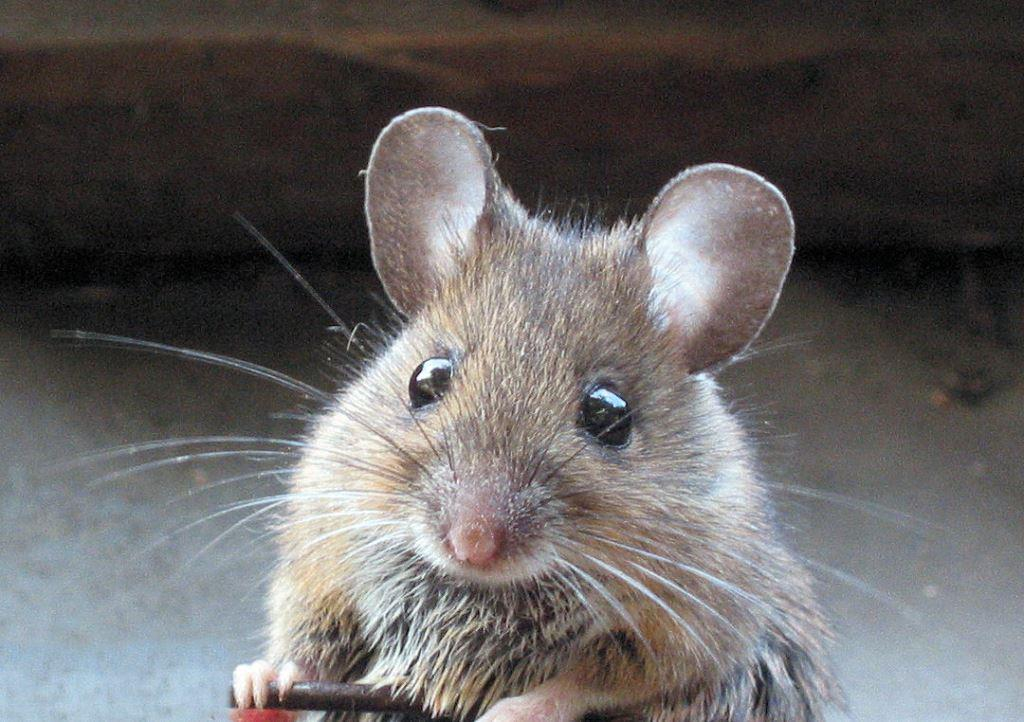
\includegraphics[width=\textwidth]{files/images/mouse}
%                \caption{A mouse}
%                \label{fig:mouse}
%        \end{subfigure}
%        \caption{Pictures of animals}\label{fig:animals}
%\end{figure}
%
%
%
%\subsection{subsection name}
%
%On the other hand, the authors of \cite{2004_Whitesides_writing_a_paper} argue that: \lipsum[4] 



% To gather acronyms or explain some technical mumbo jumbo, a nomenclature may come in handy :)
% you can create hyperlinks between acronyms in the bulk text and their descriptions, which are placed inside this nomenclature-chapter

% the "*" after "chapter" is used to suppress the chapter number
\chapter*{Nomenclature}   

% include Nomenclature into the table of contents
\addcontentsline{toc}{chapter}{Nomenclature}

% add label to reference to nomenclature
\label{text:nomenclature}

% The nomenclature can be divided into different categories, e.g. via sections
\section*{Abbreviations}

\begin{acronym}[$leeeeeeength_of_tabulator$]    % number of "eee"s defines the length of tabulator between acronym and its explanation
\setlength{\itemsep}{0mm}

% now the acronyms can be defined, syntax:
% \acro{input for \ac{..} }[displayed form]{\acroextra{\hyperref[label at first occurrence]{long form, shown only here}}}

% sample data
\acro{tg}[TG]{\acroextra{\hyperref[def:tg]{Thermogravimetry}}}


\end{acronym}

% to place the acronym inside the text, you can write one of the following:
% \ac{..}   % initially full, then short form
% \acf{..}  % full form
% \acs{..}  % short form


% Normally, any \label outside an object (like figures or tables) points to the current section title.
% To have a link point to the exact line where the \label is defined (e.g. to point exactly to the first usage of a new acronym), you can use the command \phantomsection just before the label and acronym
%% bla bla
%% \phantomsection \label{def:tg} \acs{tg}
%% bla bla


\section*{Greek Symbols}
\begin{acronym}[$leeeeeeength_of_tabulator$]
\setlength{\itemsep}{0mm}

%% start listing acronyms
\acro{eps}[$\epsilon$]{\acroextra{\hyperref[def:eps]{Die Permittivität $\epsilon$, auch bekannt als dielektrische Konstante, ist ein Mass für die Durchlässigkeit eines Materials für elektrische Felder.}}}

% to check if symbols not used in the text are omitted from the nomenclature, an additional entry is placed here:
\acro{om}[$\omega$]{\acroextra{\hyperref[def:om]{Elektrischer Widerstand in [Ohm].}}}

\end{acronym} 

% The bibliography is usually put at the end of a report
% set a smaller font size for references
\begin{footnotesize}

% increase space between individual text lines for readability
\begingroup\linespread{1.2}\selectfont

% in order to break long URLs into several lines, add option to execute \linebreak after "/" (default) and additionally "-" 
\def\UrlBigBreaks{\do\/\do-}

%bibstyle refers to a file bibstyle.bst, which defines how your citations will look
% assign output style to bibliography
\bibliographystyle{files/bibliography/unsrturl}

% unsrt stands for "unsorted", i.e. don't sort references in alphabetical order but put them in the order of citation instead

% access the bibtex bibliography file
%Only the entries referred to via \cite and \nocite will be listed in the bibliography.
\bibliography{files/bibliography/references}

% if references are printed in the wrong order
% --> delete the file "bibliography.bib.bak" and compile again

\endgroup

\end{footnotesize}



%\begin{thebibliography}{widest-label}
%\bibitem[label]{cite_key}
%...
%\end{thebibliography}

% To implement a custom bibliography style with the citations in order of appearance and allowing for urls, the file "unsrturl.bst" has to be located in the same folder as the main .tex-file (=in our case "report.tex").

%% template for a scientific report:
%% you can create hyperlinks between acronyms in the bulk text and their descriptions, which are placed inside this nomenclature-chapter

% the "*" after "chapter" is used to suppress the chapter number
\chapter*{Nomenclature}   

% include Nomenclature into the table of contents
\addcontentsline{toc}{chapter}{Nomenclature}

% add label to reference to nomenclature
\label{text:nomenclature}

% The nomenclature can be divided into different categories, e.g. via sections
\section*{Abbreviations}

\begin{acronym}[$leeeeeeength_of_tabulator$]    % number of "eee"s defines the length of tabulator between acronym and its explanation
\setlength{\itemsep}{0mm}

% now the acronyms can be defined, syntax:
% \acro{input for \ac{..} }[displayed form]{\acroextra{\hyperref[label at first occurrence]{long form, shown only here}}}

% sample data
\acro{tg}[TG]{\acroextra{\hyperref[def:tg]{Thermogravimetry}}}


\end{acronym}

% to place the acronym inside the text, you can write one of the following:
% \ac{..}   % initially full, then short form
% \acf{..}  % full form
% \acs{..}  % short form


% Normally, any \label outside an object (like figures or tables) points to the current section title.
% To have a link point to the exact line where the \label is defined (e.g. to point exactly to the first usage of a new acronym), you can use the command \phantomsection just before the label and acronym
%% bla bla
%% \phantomsection \label{def:tg} \acs{tg}
%% bla bla


\section*{Greek Symbols}
\begin{acronym}[$leeeeeeength_of_tabulator$]
\setlength{\itemsep}{0mm}

%% start listing acronyms
\acro{eps}[$\epsilon$]{\acroextra{\hyperref[def:eps]{Die Permittivität $\epsilon$, auch bekannt als dielektrische Konstante, ist ein Mass für die Durchlässigkeit eines Materials für elektrische Felder.}}}

% to check if symbols not used in the text are omitted from the nomenclature, an additional entry is placed here:
\acro{om}[$\omega$]{\acroextra{\hyperref[def:om]{Elektrischer Widerstand in [Ohm].}}}

\end{acronym} 
%\input{files/chapters/Motivation}
%\input{files/chapters/Previous_Work}
%\input{files/chapters/Experimental_Setup}
%\input{files/chapters/Materials_and_Methods}
%\input{files/chapters/Results}
%\input{files/chapters/Discussion}
%\input{files/chapters/Conclusion}
%\input{files/chapters/Outlook}
%% set a smaller font size for references
\begin{footnotesize}

% increase space between individual text lines for readability
\begingroup\linespread{1.2}\selectfont

% in order to break long URLs into several lines, add option to execute \linebreak after "/" (default) and additionally "-" 
\def\UrlBigBreaks{\do\/\do-}

%bibstyle refers to a file bibstyle.bst, which defines how your citations will look
% assign output style to bibliography
\bibliographystyle{files/bibliography/unsrturl}

% unsrt stands for "unsorted", i.e. don't sort references in alphabetical order but put them in the order of citation instead

% access the bibtex bibliography file
%Only the entries referred to via \cite and \nocite will be listed in the bibliography.
\bibliography{files/bibliography/references}

% if references are printed in the wrong order
% --> delete the file "bibliography.bib.bak" and compile again

\endgroup

\end{footnotesize}



%\begin{thebibliography}{widest-label}
%\bibitem[label]{cite_key}
%...
%\end{thebibliography}
%\input{files/chapters/Appendix}

% end the document
\end{document} 